% With the observation that ribosomes set an inherent upper limit on growth
% rate, through both rRNA synthesis and the additional dependence on ribosomal
% fraction, it is also plausible that ribosomes may play a more dominant role
% in setting growth rate across other growth conditions. With a rich proteomic
% data set across a wide array of conditions, and in light of a number of
% recent experimental observations, we find that cells also appear to tune
% their ribosomal abundance as a means to maximize growth even in poor nutrient
% conditions. This has important consequences on the relationship with cell
% size and maintenance of steady-state growth. In the coming section and the
% remainder of the text, we consider these further beginning with cell size.

\subsection{Relationship Between Cell Size and Growth Rate}
The relationship between cell size and growth rate has long been of interest in
the study of bacterial physiology, particularly following the now six decade-old
observation that cell volume appears to increase exponentially with growth rate;
known as Schaechter's growth law \citep{schaechter1958, taheriaraghi2015}.
However, the mechanism that governs this relationship, and even the question of
whether the change in average cell size is truly exponential, has remained under
debate \citep{harris2018}.  Here we examine the influence of ribosomal conrtent
and total protein abundance on cell size.

As shown in \FIG{ribosome_limit}(C), cells grow at a near-maximal rate dictated
by their total ribosomal mass fraction $\Phi_R$, at least at moderate growth
rates above 0.5 hr$^{-1}$ (where $f_a$ is close to 1). Here,  growth rate can be
increased only by making more ribosomes in a way that increases  $\Phi_R$. As
\textit{E. coli} grows faster, however, large swaths of the proteome also
increase in absolute protein, and the ability to add additional ribosomes is
likely constrained by others factors such as  crowding due to their large size
\citep{delarue2018, solerbistue2020}. It is now well-documented that
\textit{E. coli} cells add a constant volume per origin of replication (termed a
"unit cell" or "initiation mass"), which is robust to a remarkable array of
cellular perturbations \citep{si2017}. To consider this dependency in the context of the
proteomic data, we used measurements from \cite{si2017} for wild-type
\textit{E. coli} cells grown in different nutrient conditions
(\FIG{translation_ecoli_partA}(A)) to estimate the average number of origins per
cell $\langle$\# ori$\rangle$ across the data.

The average number of origins $\langle$\# ori$\rangle$ is set by how often
replication must be initiated per cell doubling under steady-state growth.
This can be quantified as
\begin{equation}
    \langle \text{\# ori} \rangle = 2^{\tau_{cyc} / \tau} = 2^{\tau_{cyc} \lambda / ln(2)},
    \label{eq:Nori}
\end{equation}
where $t_{cyc}$ is the cell cycle time (referring to the time from replication
initiation to cell division), and $\tau$ is the cell doubling time. For
ribosomal synthesis, we find an approximately linear correlation between
ribosome copy number and $\langle$\# ori$\rangle$
(\FIG{translation_ecoli_partA}(B)). For a constant cell cycle time, observed at
growth rates above about 0.5 hr$^{-1}$ \citep{helmstetter1968}, \EQ{Nori} states
that $\langle \text{\# ori} \rangle$ will need to increase exponentially with
the growth rate in order to maintain steady-state growth.


Why does \textit{E. coli} add a constant volume per $\langle$\# ori$\rangle$?
To consider how this trend pertains to growth, we must consider
how the proteome size and composition changes with respect to growth rate. In
\FIG{translation_ecoli_partA}(D), we analyze the position-dependent protein
expression across the chromosome for each of the growth conditions from
\cite{schmidt2016}. Here, we have calculated a running Gaussian average of
protein copy number (20 kbp st. dev. averaging window) based on each gene's
transcriptional start site, which were then median-subtracted to account for the
differences in total protein abundance with each growth condition. Importantly,
we find that the major deviations in protein copy number are largely restricted
to regions of ribosomal protein genes, with substantially higher deviations
observed for cells with high $\langle$\# ori$\rangle$ (teal), as compared to
those with low $\langle$\# ori$\rangle$ (purple). This is particularly apparent
for genes closer to the origin, where the majority of ribosomal proteins are
found. This suggests that in addition to the linear scaling between protein
abundance and $\langle$\# ori$\rangle$, the relative ribosomal abundance is
tuned in proportion to $\langle$\# ori$\rangle$.  Given the increased rRNA gene
dosage required at faster growth rates, additional rounds of DNA replication
have the effect of skewing DNA dosage in favor of additional ribosomal synthesis
Since growth rate depends specifically on the ribosomal fraction $\Phi_R$, this
result suggests that cells are changing their size as a way to vary the absolute
number of ribosomes per cell andtune $\Phi_R$ according to better match
available nutrient conditions.


\begin{figure*}
    \begin{fullwidth}
    \centering{
        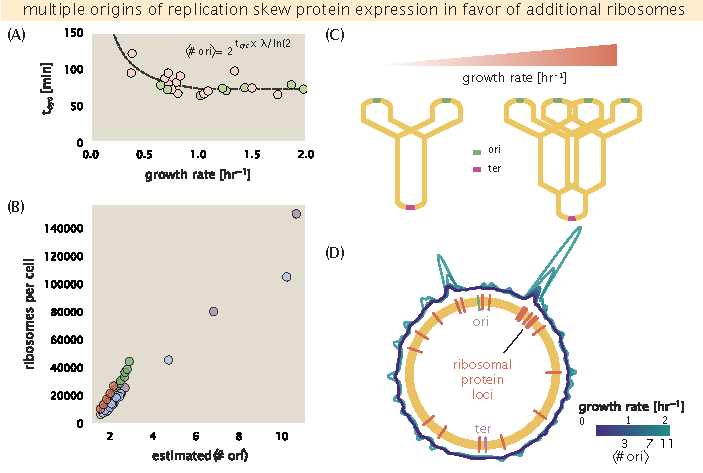
\includegraphics{main_figs/fig8_ribosome_growth_limit_ecoli_a_polar_coord.pdf}
        \caption{\textbf{Cells increase absolute ribosome abundance with
        $\langle$\# ori$\rangle$.} (A) Experimental data from Si \textit{et al.}
        (2017). Dashed line shows fit to the data, which were used to estimate
        $\langle$\# ori$\rangle$. $t_{cyc}$ was assumed to vary in proportion to
        $\tau$ for doubling times great than 40 minutes, and then reach a
        minimum value of 73 minutes below this (see Appendix
        \nameref{sec:SI_ori} for additional details). Red data points correspond
        to measurements in strain MG1655, while light green points are for
        strain NCM3722. (B) Plot of the ribosome copy number estimated from the
        proteomic data against the estimated $\langle$\# ori$\rangle$. (C)
        Schematic shows the expected increase in replication forks (or number of
        ori regions) as \textit{E. coli} cells grow faster. (D) A running
        Gaussian average (20 kbp st. dev.) of protein copy number is calculated
        for each growth condition considered by \citep{schmidt2016}. Since total
        protein abundance increases with growth rate, protein copy numbers are
        median-subtracted to allow comparison between growth conditions.
        $\langle$\# ori$\rangle$ are estimated using the data in (A) and
        Equation \ref{eq:Nori}. } \label{fig:translation_ecoli_partA}
    }
    \end{fullwidth}
\end{figure*}
